\documentclass[12pt]{article}
\usepackage{sbc-template}
\usepackage{graphicx,url}
\usepackage{enumitem}
\usepackage[utf8]{inputenc}
\usepackage[brazil]{babel}
\usepackage[latin1]{inputenc}

\sloppy

\title{Inteligência artificial aplicada à detecção e classificação de animais em ambiente confinado}

\author{Vinícius L. Gonçalves\inst{1}, Luciana Conceição D. Campos\inst{1}, Érica da Costa R. Carvalho\inst{2} }


\address{Departamento de Ciência da Computação -- Universidade Federal de Juiz de Fora
  (UFJF)\\
  José Lourenço Kelmer, Juiz de Fora, MG, 36036-900, Brasil
\nextinstitute
  Departamento de Ciência da Computação -- Universidade Federal de São João del-Rei (UFSJ)\\
  Av. Visc. do Rio Preto, S/N - Fábricas, São João del-Rei, MG, 36301-360, Brasil
  \email{ vinicius.latini@estudante.ufjf.br, luciana.campos@ufjf.br}
  \email{ ericacarvalho@ufsj.edu.br }
}

\include{Template_SBC/common}

\begin{document} 

\maketitle

% \begin{abstract}
%   This project proposes the development of a low-cost system based on Computer Vision and Artificial Intelligence for the detection and behavioral classification of confined \textit{Saanen} goats. The initiative integrates knowledge from the fields of Computer Science and Animal Science, using videos captured in experimental environments to build a labeled image dataset. Machine learning models will be trained to identify behavioral patterns of the goats and compare these predictions with previously annotated results. In this way, the project aims to create a tool that can support both the monitoring and study of these animals.
% \end{abstract}
     
\begin{resumo} 
  O presente trabalho propõe o desenvolvimento de um sistema de baixo custo baseado em Visão Computacional e Inteligência Artificial para detecção e classificação de cabras da raça \textit{Saanen} em confinamento. A proposta iniciativa integra conhecimentos das áreas de Ciência da Computação e Zootecnia, utilizando vídeos capturados em ambientes experimentais para a construção de um banco de imagens rotuladas. Modelos de aprendizado de máquina serão treinados para identificar os caprinos e comparar essas predições com os resultados anotados previamente. Dessa forma, espera-se construir uma ferramenta que possa auxiliar tanto na detecção quanto na classificação desses animais.
\end{resumo}


\section{Introdução}
\label{sec:introducao}

\subsection{Contextualização}
\label{subsec:contextualizacao}

O uso de sistemas baseados em Visão Computacional (VC) e Inteligência Artificial (IA) tem se expandido consideravelmente nos últimos anos, especialmente no contexto da agricultura de precisão e do manejo zootécnico \cite{kamilaris2018deep}. Essas tecnologias vêm possibilitando o desenvolvimento de soluções inovadoras para o controle de atividades em ambientes rurais e experimentais, com aplicações que vão desde a inspeção de qualidade \cite{industrial_quality_cv_2024}, a análise de comportamento animal \cite{animalformer_2024} e o monitoramento de cultivos \cite{vit_precision_agriculture_2025}, até a automação de processos \cite{kang2025bokchoy_cv_iot}. Por serem acessíveis, precisas e não invasivas, tais inovações contribuem para a adoção de práticas mais eficientes e sustentáveis.

Na produção animal, esse movimento é conhecido como Zootecnia de Precisão (\textit{Precision Livestock Farming} -- PLF), cuja proposta é monitorar os animais de forma contínua e automatizada, gerando informação em tempo hábil para apoiar a tomada de decisão do produtor e do pesquisador \cite{berckmans2014plf}. Um dos aspectos fundamentais para o bem-estar animal na pecuária é a garantia de um ambiente adequado, com alimentação e água em quantidade e qualidade suficientes, o que demanda uma quantidade significativa de horas de trabalho humano de observação. Com o avanço da ciência e da tecnologia, bem como com o aumento das exigências dos consumidores por produtos de origem animal de alta qualidade, torna-se cada vez mais necessário o aprimoramento dos métodos de monitoramento da produção pecuária \cite{dominiak2019, nasirahmadi2017, halachmi2019}. A integração de sensores, grandes volumes de dados e aprendizado de máquina tem possibilitado a obtenção e a interpretação dessas informações de forma mais eficiente \cite{neethirajan2020sensors}, e diversas pesquisas já demonstraram a viabilidade do monitoramento automático do comportamento animal, frequentemente aliado à análise de características comportamentais e fisiológicas \cite{halachmi2019, fogarty2018, rohan2023deep_livestock_survey}.

Entre as modalidades de sensoriamento disponíveis, as câmeras de vídeo ocupam posição de destaque por serem não invasivas -- dispensam qualquer dispositivo fixado ao corpo do animal -- e por permitirem que uma única instalação observe vários indivíduos simultaneamente \cite{nasirahmadi2017}. Em quase todas as aplicações de monitoramento por vídeo, a primeira etapa do processamento é a \textbf{detecção} dos animais, isto é, a localização de cada indivíduo na imagem por meio de uma caixa delimitadora (\textit{bounding box}). É sobre a saída do detector que se constroem as etapas posteriores, como a contagem do rebanho, o rastreamento individual ao longo do tempo e a classificação de comportamentos (alimentação, ócio, deslocamento, interação). Um detector impreciso propaga seus erros para toda a cadeia de análise, de forma que a qualidade dessa etapa condiciona a utilidade do sistema como um todo.

\subsection{Motivação e Definição do Problema}
\label{subsec:motivacao}

Na Universidade Federal de São João del-Rei (UFSJ), essa abordagem está sendo explorada no projeto interdisciplinar ``Inteligência artificial aplicada à detecção e classificação comportamental de cabras em confinamento (raça \textit{Saanen})'', que envolve docentes e discentes dos cursos de Zootecnia e Ciência da Computação da UFSJ, em parceria com a Universidade Federal de Juiz de Fora (UFJF). No âmbito desse projeto, um rebanho de oito cabras da raça \textit{Saanen} é mantido em uma baia experimental monitorada por quatro câmeras fixas, que registram os animais sob duas perspectivas -- \textbf{frontal} e \textbf{superior} (zenital) -- e sob duas condições de iluminação -- \textbf{diurna}, com luz natural, e \textbf{noturna}, com imagem em espectro infravermelho. O presente trabalho corresponde ao módulo de detecção desse projeto guarda-chuva e fornece a base sobre a qual as etapas de análise comportamental poderão ser desenvolvidas.

Apesar da ampla disponibilidade de recursos tecnológicos, aplicar esses sistemas em um ambiente real de confinamento impõe desafios que não aparecem em bases de dados de propósito geral. O primeiro deles é a ausência de modelos prontos para a espécie-alvo. Detectores de objetos modernos, como os da família YOLO (\textit{You Only Look Once}) \cite{redmon2016yolo, jocher2023yolov8}, são distribuídos com pesos pré-treinados no conjunto COCO (\textit{Common Objects in Context}) \cite{journals/corr/LinMBHPRDZ14}, que não possui uma classe para caprinos. Em um teste preliminar realizado neste trabalho, utilizando o YOLOv8 pré-treinado e a classe morfologicamente mais próxima disponível (\textit{sheep}, ovelha), o modelo identificou apenas dois dos oito animais presentes na baia, com confianças de 0,27 e 0,48, e apresentou comportamento igualmente insatisfatório em imagens noturnas e na perspectiva superior. Esse resultado evidenciou a necessidade de construir uma base de imagens rotuladas própria e de treinar detectores específicos para o domínio. A construção dessa base, por sua vez, é custosa: exige a extração de quadros dos vídeos, a anotação manual de dezenas de milhares de caixas delimitadoras e conhecimento técnico para organizar os dados no formato exigido pelos modelos.

O segundo desafio é a \textbf{heterogeneidade das condições de captura}. Uma mesma cabra tem aparência muito diferente quando vista de frente ou de cima, e as imagens noturnas em infravermelho são monocromáticas, com contraste e textura distintos das imagens diurnas coloridas. Na vista superior, os animais aparecem menores e frequentemente agrupados em torno do cocho, com oclusão parcial entre indivíduos. Um único detector treinado sobre todas essas condições precisa acomodar, em um mesmo conjunto de parâmetros, distribuições visuais bastante diferentes entre si, o que pode se manifestar como detecções perdidas em um cenário e detecções duplicadas em outro.

O terceiro desafio é de natureza metodológica e diz respeito à \textbf{avaliação} dos modelos. Como as imagens são quadros extraídos de vídeos contínuos, quadros vizinhos de uma mesma gravação são praticamente idênticos. Um particionamento aleatório entre treino e validação, como o da validação cruzada \textit{K-Fold} convencional, tende a colocar quadros quase duplicados nos dois conjuntos, caracterizando vazamento de dados (\textit{data leakage}) \cite{kaufman2012leakage}: o modelo passa a ser avaliado sobre amostras dependentes das que viu no treinamento, e as métricas passam a medir memorização em vez de capacidade de generalização. Dados com estrutura temporal exigem estratégias de particionamento que respeitem essa estrutura \cite{roberts2017crossvalidation}. Esse risco se manifestou nas primeiras rodadas de experimentos deste trabalho, que utilizavam particionamento aleatório e produziram métricas muito próximas do máximo, levantando a suspeita de vazamento e motivando a revisão do protocolo de validação.

Diante desse cenário, este trabalho procura responder à seguinte questão: \textit{é possível detectar de forma robusta caprinos em um ambiente de confinamento sujeito a variações de perspectiva e iluminação, organizando o problema em detectores especializados por condição de captura, e como essa organização se compara a um único detector treinado sobre todas as condições, sob um protocolo de avaliação que reduza o vazamento temporal?}

\subsection{Proposta}
\label{subsec:proposta}

Para enfrentar a heterogeneidade das condições de captura, propõe-se uma arquitetura baseada em Mistura de Especialistas (\textit{Mixture of Experts} -- MoE). O conceito, introduzido no início da década de 1990 \cite{jacobs1991adaptive}, parte do princípio de ``dividir para conquistar'': o espaço de entradas é dividido entre vários modelos especialistas, e uma rede de roteamento (\textit{gating network}) decide qual especialista deve tratar cada entrada. Quando apenas um especialista é ativado por entrada (roteamento esparso), a capacidade total do sistema cresce sem que o custo de inferência cresça na mesma proporção \cite{shazeer2017outrageously}.

Na arquitetura proposta, a rede de roteamento é uma rede neural convolucional leve, a EfficientNet-B0 \cite{tan2019efficientnet}, cuja única função é classificar o \textbf{cenário de captura} -- Frontal Dia, Frontal Noite, Superior Dia ou Superior Noite -- a partir do primeiro quadro do vídeo. Ressalta-se que a rede de roteamento não classifica os animais: ela identifica o contexto da cena e, com base nele, ativa um dentre quatro detectores YOLOv8 \cite{jocher2023yolov8} especializados, cada qual treinado exclusivamente com imagens de uma combinação de perspectiva e iluminação e responsável pela detecção da classe única \texttt{goat}. Para verificar se a rede de roteamento baseia suas decisões em características do ambiente, e não em artefatos espúrios, sua decisão é analisada por meio de mapas de sensibilidade por oclusão \cite{zeiler2014visualizing}.

A arquitetura é avaliada em comparação direta com um \textbf{baseline monolítico}: um único YOLOv8 treinado sobre a união das imagens dos quatro cenários, submetido aos mesmos hiperparâmetros e ao mesmo protocolo de validação cruzada por blocos temporais contíguos, com zona de purga entre treino e validação. Dessa forma, a comparação isola o efeito da especialização, e não o de diferenças de protocolo experimental.

\subsection{Objetivos}
\label{subsec:objetivos}

\subsubsection*{Objetivo geral}

Desenvolver e avaliar uma arquitetura baseada em Mistura de Especialistas, composta por uma rede de roteamento que identifica o cenário de captura e por detectores YOLOv8 especializados, para a detecção automatizada de caprinos da raça \textit{Saanen} em ambiente de confinamento sujeito a variações de perspectiva (frontal e superior) e de iluminação (diurna e noturna).

\subsubsection*{Objetivos específicos}

\begin{enumerate}[label=\roman*.]
    \item Construir e caracterizar uma base de imagens rotuladas com a classe única \texttt{goat}, a partir de vídeos capturados em ambiente experimental de confinamento, contemplando os quatro cenários de captura;
    \item Definir um protocolo de validação cruzada por blocos temporais contíguos, com zona de purga entre treino e validação, que reduza o vazamento de dados decorrente da correlação entre quadros consecutivos de vídeo;
    \item Treinar e avaliar quatro detectores YOLOv8 especializados, um para cada combinação de perspectiva e iluminação;
    \item Treinar uma rede de roteamento baseada em EfficientNet-B0 para a classificação do cenário de captura e analisar, por meio de sensibilidade por oclusão, as regiões da imagem que fundamentam suas decisões;
    \item Integrar a rede de roteamento e os especialistas em um \textit{pipeline} único de inferência sobre vídeo;
    \item Comparar a arquitetura proposta com um detector monolítico treinado sobre todos os cenários, tanto por métricas agregadas de detecção (Precisão, Revocação, F1, mAP50 e mAP50-95) quanto pela estabilidade da contagem de animais em vídeos de teste independentes.
\end{enumerate}

\subsection{Justificativa}
\label{subsec:justificativa}

A justificativa para este trabalho está na importância de desenvolver tecnologias que auxiliem no monitoramento de animais em confinamento de forma automatizada, precisa e não invasiva. A observação visual contínua de um rebanho é uma tarefa repetitiva e demorada, sujeita à fadiga do observador, e se torna ainda mais difícil no período noturno. Um detector confiável reduz o esforço manual envolvido nesse acompanhamento e constitui o componente de base para as análises de interesse zootécnico previstas no projeto, como a contagem, o rastreamento e a classificação comportamental dos animais.

Do ponto de vista científico, o trabalho contribui com uma base de imagens de caprinos anotada e organizada por condição de captura -- recurso escasso na literatura, que concentra os estudos em bovinos e suínos \cite{nasirahmadi2017, rohan2023deep_livestock_survey} -- e com um protocolo de avaliação que trata explicitamente o vazamento temporal, problema frequente em trabalhos que utilizam quadros extraídos de vídeo. Além disso, investiga-se se a especialização por contexto, organizada na forma de uma Mistura de Especialistas, oferece vantagens em relação a um detector único, uma pergunta de interesse para aplicações em que as condições de captura variam de forma previsível, como é o caso de câmeras fixas operando ao longo do dia e da noite.

Do ponto de vista prático, a arquitetura modular facilita a manutenção e a expansão do sistema: a inclusão de um novo cenário de captura (por exemplo, uma nova câmera ou uma nova baia) requer apenas o treinamento de um novo especialista e a atualização da rede de roteamento, sem retreinar os especialistas existentes. Por fim, o trabalho está em consonância com a Agenda 2030 da Organização das Nações Unidas, especialmente com os Objetivos de Desenvolvimento Sustentável 2 (Fome Zero e Agricultura Sustentável), 9 (Indústria, Inovação e Infraestrutura) e 12 (Consumo e Produção Responsáveis), ao propor uma ferramenta tecnológica voltada ao monitoramento de caprinos com foco em bem-estar animal e produtividade sustentável.

\subsection{Escopo e Delimitação}
\label{subsec:escopo}

Para evitar ambiguidades, delimita-se a seguir o que está e o que não está no escopo deste trabalho:

\begin{itemize}
    \item \textbf{Tarefa:} detecção de objetos com classe única (\texttt{goat}), ou seja, localização de cada animal por uma caixa delimitadora. Não são realizadas a classificação comportamental, a identificação individual dos animais nem o rastreamento ao longo do tempo (\textit{multi-object tracking}), que permanecem como direções de trabalhos futuros no projeto guarda-chuva.
    \item \textbf{Papel da classificação:} a única etapa de classificação presente na arquitetura é a da rede de roteamento, que classifica o cenário de captura (perspectiva e iluminação) e não os animais.
    \item \textbf{Domínio dos dados:} uma única baia experimental da UFSJ, com um rebanho de oito cabras da raça \textit{Saanen}, registrada por quatro câmeras fixas. A generalização para outras instalações, raças ou espécies não é avaliada.
    \item \textbf{Roteamento:} a rede de roteamento opera uma vez por vídeo, a partir do primeiro quadro, e ativa um único especialista (roteamento rígido, \textit{top-1}). Transições de cenário dentro de um mesmo vídeo não são tratadas.
    \item \textbf{Plataforma de execução:} os experimentos foram conduzidos em uma estação de trabalho com GPU dedicada. A implantação e a medição de desempenho em \textit{hardware} embarcado de baixo custo não fazem parte deste trabalho.
\end{itemize}

\subsection{Contribuições}
\label{subsec:contribuicoes}

As principais contribuições deste trabalho são:

\begin{enumerate}
    \item Uma base de imagens de caprinos da raça \textit{Saanen} em confinamento, com 8.604 imagens e 66.705 caixas delimitadoras anotadas, provenientes de 36 sessões de gravação e organizadas nos quatro cenários de captura;
    \item Um protocolo de validação cruzada por blocos temporais contíguos com zona de purga, acompanhado de auditoria do particionamento, aplicado de forma idêntica aos especialistas e ao baseline;
    \item Uma arquitetura de Mistura de Especialistas para detecção, com rede de roteamento interpretável por análise de oclusão, integrada em um \textit{pipeline} de inferência sobre vídeo;
    \item Uma comparação experimental entre a arquitetura proposta e um detector monolítico treinado nas mesmas condições. Os resultados mostram que as duas abordagens atingem desempenho elevado e semelhante nas métricas agregadas de validação (mAP50 próximo de 0,995 em ambas), mas que, em vídeos de teste independentes, os especialistas mantiveram a contagem correta dos oito animais em todos os quadros dos quatro cenários, enquanto o modelo monolítico apresentou subdetecção em alguns cenários e detecções duplicadas em outros.
\end{enumerate}

\subsection{Organização do Trabalho}
\label{subsec:organizacao}

O restante deste trabalho está organizado da seguinte forma. A Seção~2 apresenta a fundamentação teórica necessária à compreensão da proposta: redes neurais convolucionais, detecção de objetos e a família YOLO, a arquitetura EfficientNet, o paradigma de Mistura de Especialistas, as métricas de avaliação de detectores, a validação cruzada e o problema de vazamento de dados, e as técnicas de explicabilidade por oclusão. A Seção~3 discute os trabalhos relacionados ao uso de visão computacional na pecuária de precisão, com ênfase na detecção de pequenos ruminantes. A Seção~4 descreve os materiais e métodos: a aquisição dos vídeos, a construção e a caracterização da base de imagens, o protocolo de validação por blocos temporais, a configuração dos modelos e a arquitetura MoE proposta. A Seção~5 apresenta e discute os resultados obtidos, desde a prova de conceito inicial até a comparação entre a arquitetura proposta e o baseline monolítico. Por fim, a Seção~6 apresenta as conclusões, as limitações do trabalho e as propostas de trabalhos futuros.
\todo[A numeração acima assume que os capítulos seguintes serão Fundamentação Teórica, Trabalhos Relacionados, Materiais e Métodos, Resultados e Discussão e Conclusão. Trocar os números por \textbackslash ref quando as seções existirem.]{Atualizar referências cruzadas para os capítulos seguintes.}

\section{Metodologia}

Esta seção descreve os procedimentos adotados para o desenvolvimento do presente trabalho, apresentando a fundamentação teórica para escolha da arquitetura até as etapas de coleta, tratamento de dados, treinamento e validação do modelo computacional.

\subsection{Definição da Arquitetura e Prova de Conceito}
Primeiramente, realizou-se uma pesquisa bibliográfica para definir a arquitetura do sistema, visando identificar ferramentas e abordagens eficazes para a classificação de objetos em tempo real em vídeos. Nesse contexto, selecionou-se o YOLO (\textit{You Only Look Once}), um modelo consolidado para detecção, segmentação e classificação de objetos.

A pesquisa bibliográfica concentrou-se em arquiteturas de redes neurais convolucionais (CNNs) de estágio único (single-stage detectors), comparando modelos como SSD (Single Shot Detector) e as diversas versões do YOLO. A escolha pelo YOLO justificou-se pelo seu equilíbrio superior entre custo computacional e precisão, além de sua facilidade de integração.

Com o modelo definido, desenvolveu-se uma prova de conceito (PoC) para validar o funcionamento do YOLO no cenário proposto. Este teste inicial utilizou um conjunto reduzido de \textit{frames} extraídos de gravações de caprinos, sem treinamento prévio, com o objetivo estrito de avaliar a usabilidade da ferramenta.

\subsection{Base de Dados e Rotulação}

O YOLO é fornecido como um modelo pré-treinado no conjunto de dados COCO (\textit{Common Objects in Context}). Contudo, visto que este \textit{dataset} não possui uma classe específica para caprinos, utilizou-se inicialmente a classe \textit{sheep} (ovelha) por semelhança morfológica. Como observado na Figura \ref{fig:sheep_test}, apenas duas cabras foram identificadas além da confiança da classificação ter sido baixa (0.27 e 0.48), também foram realizados outros testes variando o tipo da imagem em dia e noite e a visão utilizada, mas a classificação ainda não apresentou uma boa confiança nem identificou todos os caprinos desejados, evidenciando a necessidade de um treinamento específico com uma base de dados própria. 


\todo{Por que os resultados não foram satisfatórios? Explicar isso em forma de texto. Dizer que na figura apenas 2 cabras foram identificadas, etc.} *resolvido*
\todo{Foram testados outros vídeos ou apenas 1 para dizer que os resultados não foram satisfatórios?} *resolvido*

\begin{figure}[!h]
    \centering
    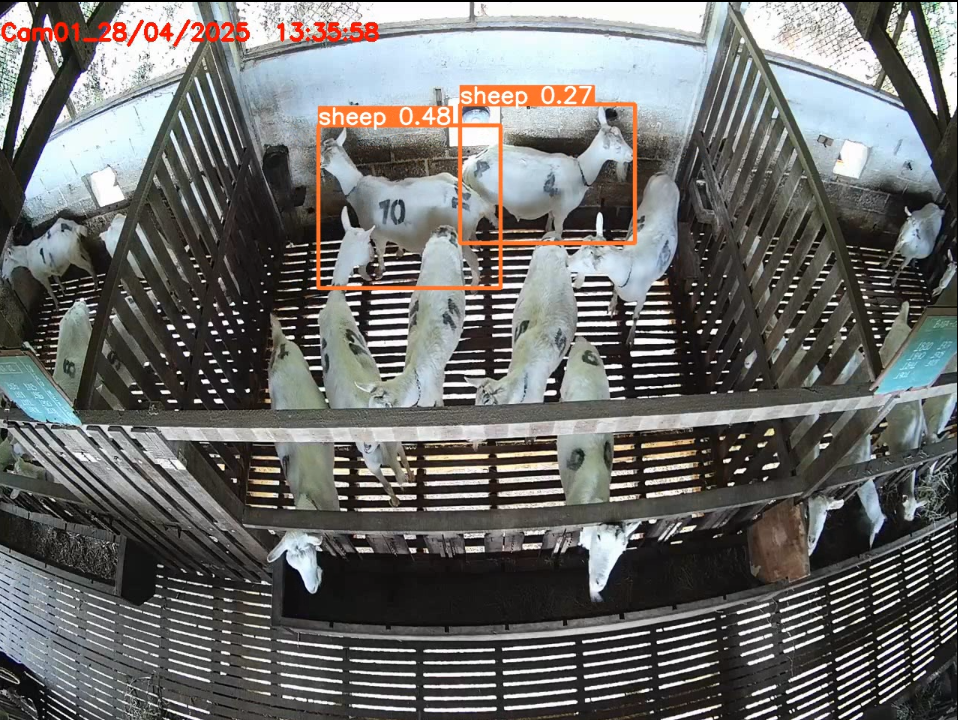
\includegraphics[width=0.8\textwidth]{./images/sheep-test.png}
    \caption{Teste realizado do modelo pre-treinado com o classe \textit{sheep}}
    \label{fig:sheep_test}
\end{figure}


Para melhorar a classificação dos animais alvo \todo{que lacuna? *resolvido*}, desenvolveu-se um \textit{script} para a extração aleatória de \textit{frames} únicos das gravações, compondo um conjunto de dados exclusivo. Dado que o YOLO opera sob o paradigma de aprendizado supervisionado, as anotações foram realizadas manualmente através da ferramenta \textit{Makesense.ai}\footnote{Disponível em: \url{https://www.makesense.ai/}}. Esta plataforma \textit{open-source} foi escolhida por permitir a rotulação em nuvem com exportação direta para o formato YOLO, facilitando o fluxo de trabalho sem necessidade de instalações locais.

O processo de rotulação seguiu um protocolo rigoroso estabelecido num guia instrutivo (ver Figuras \ref{fig:tutorial_p1} a \ref{fig:tutorial_p4}), distribuído entre colaboradores da UFSJ e voluntários da UFJF. O procedimento consistiu em cinco etapas fundamentais:
\begin{enumerate}
    \item \textbf{Carregamento e configuração:} Importação das imagens e definição da classe única denominada "goat".
    \item \textbf{Delimitação de objetos:} Aplicação de \textit{bounding boxes} apenas nos animais presentes na baia principal, ignorando áreas com fundos irrelevantes.
    \item \textbf{Refinamento:} Ajuste dos pontos de controle para garantir que as caixas envolvessem o animal de forma justa, minimizando espaços vazios.
    \item \textbf{Padronização técnica:} Cada anotação gerou uma linha num ficheiro \textit{.txt} contendo o \textit{class\_id} seguido pelas coordenadas normalizadas ($center\_x, center\_y, width, height$), conforme ilustrado no esquema de saída do YOLO.
    \item \textbf{Exportação:} Consolidação das etiquetas num ficheiro \textit{.zip} estruturado com diretórios separados para \textit{images} e \textit{labels}.
\end{enumerate}

\begin{figure}[!h]
    \centering
    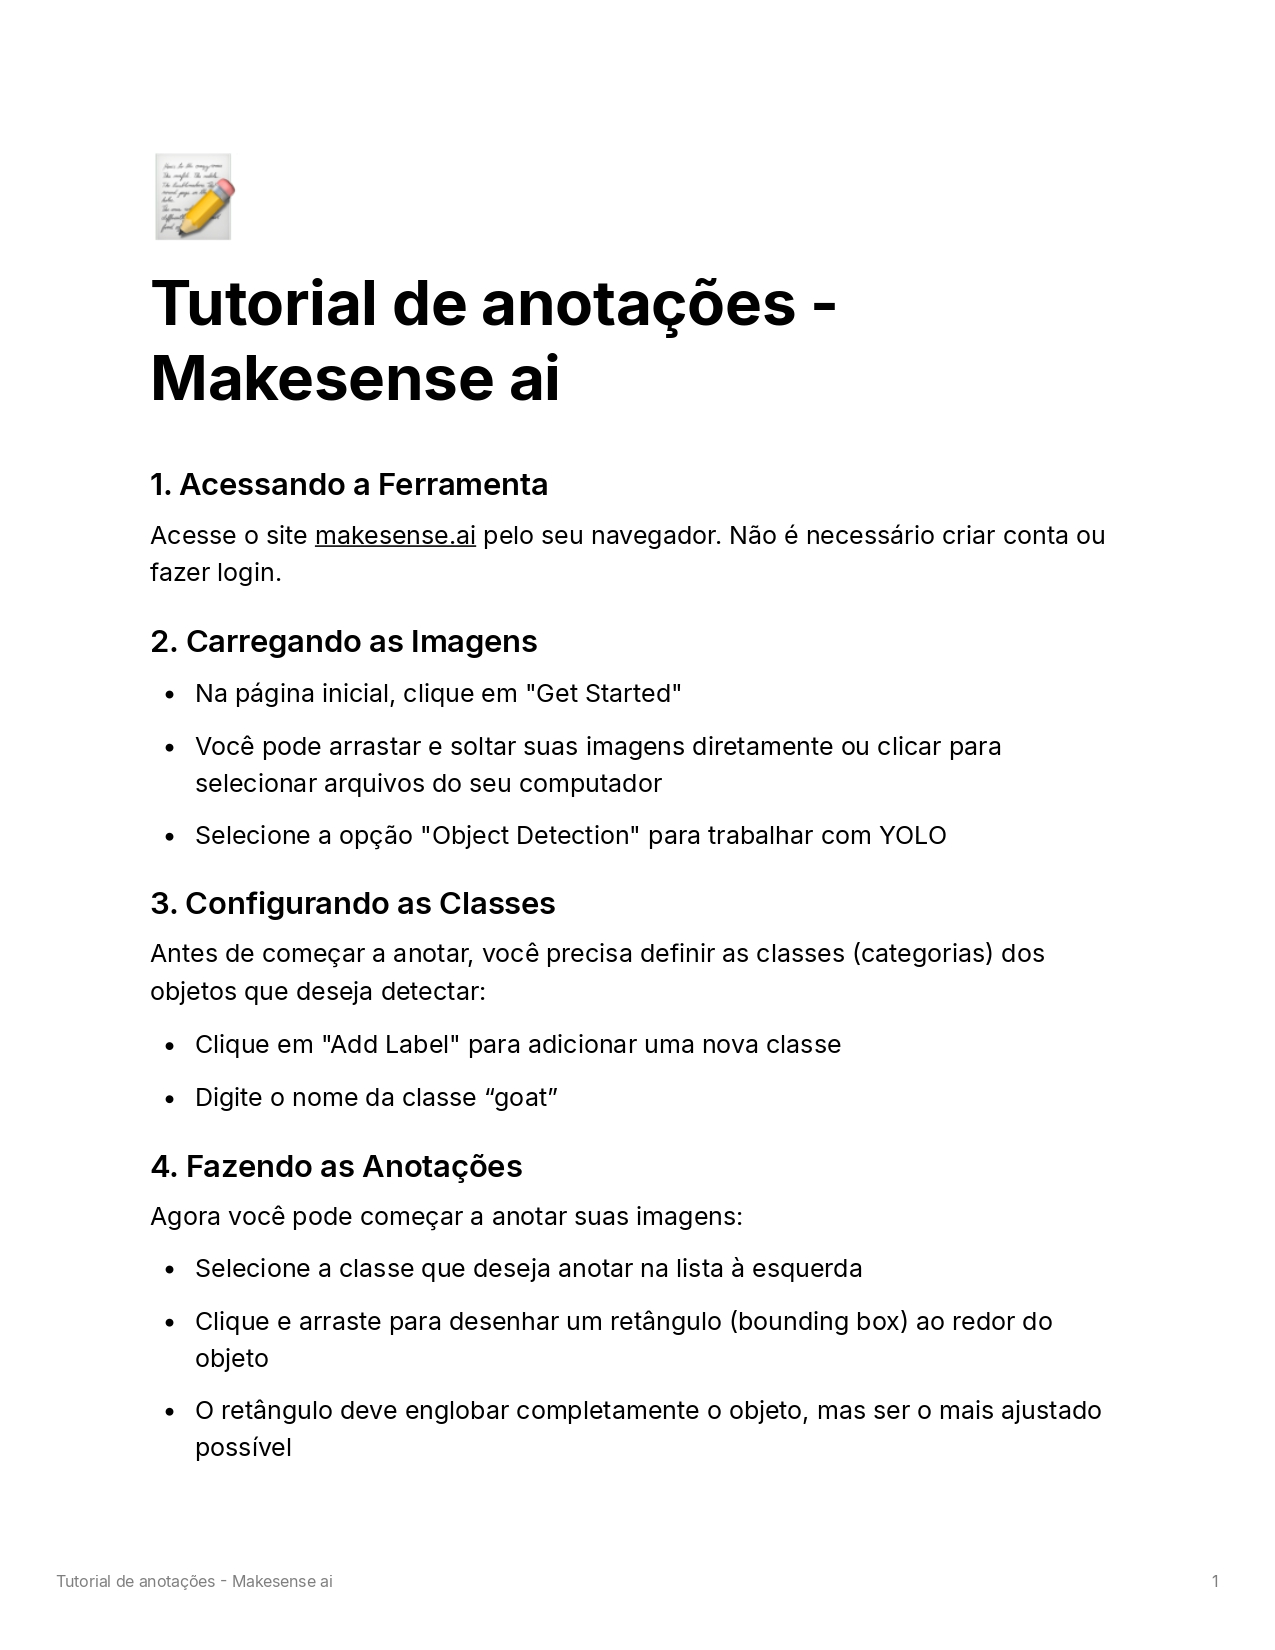
\includegraphics[width=0.8\textwidth]{./images/tutorial_p1.jpg}
    \caption{Tutorial Makesense.ai - Etapas iniciais: Carregamento e definição da classe "goat".}
    \label{fig:tutorial_p1}
\end{figure}

\begin{figure}[!h]
    \centering
    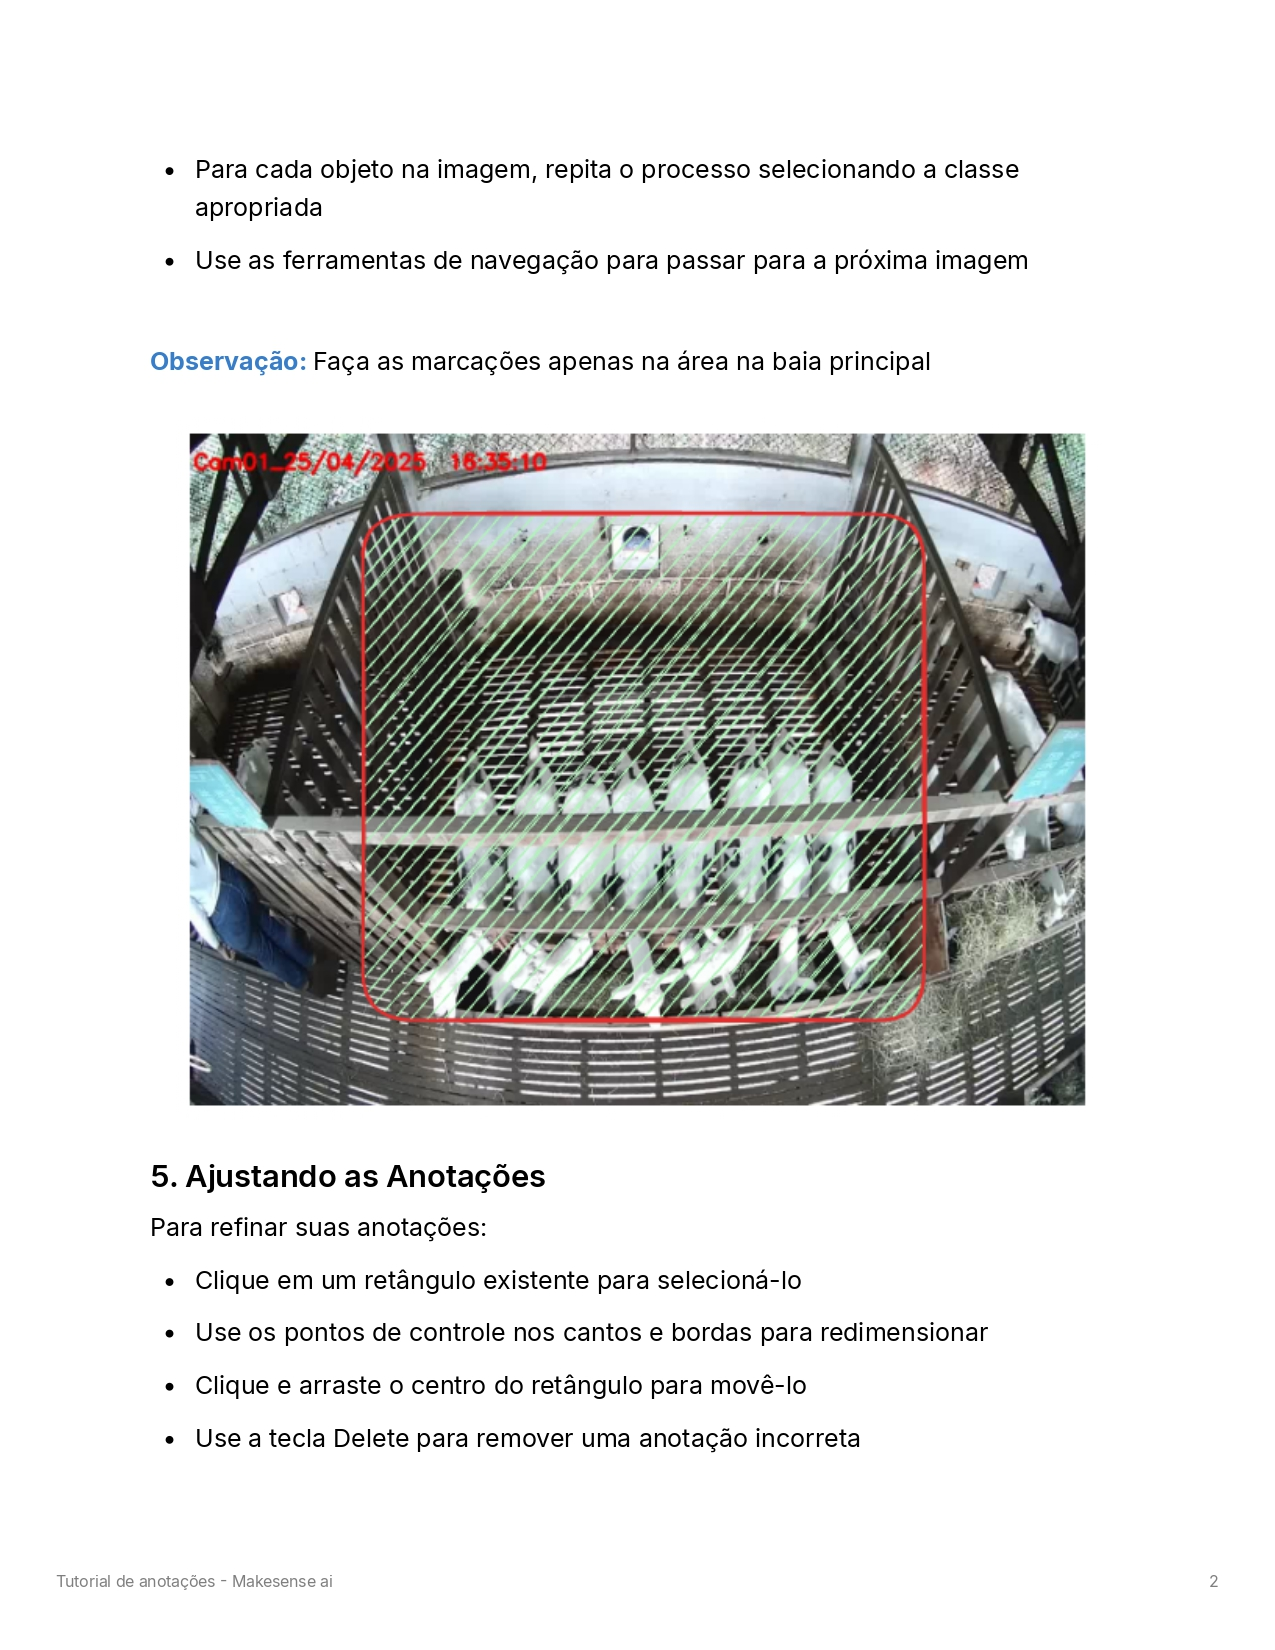
\includegraphics[width=0.8\textwidth]{./images/tutorial_p2.jpg}
    \caption{Tutorial Makesense.ai - Metodologia de marcação e restrição à baia principal.}
    \label{fig:tutorial_p2}
\end{figure}

\begin{figure}[!ht]
    \centering
    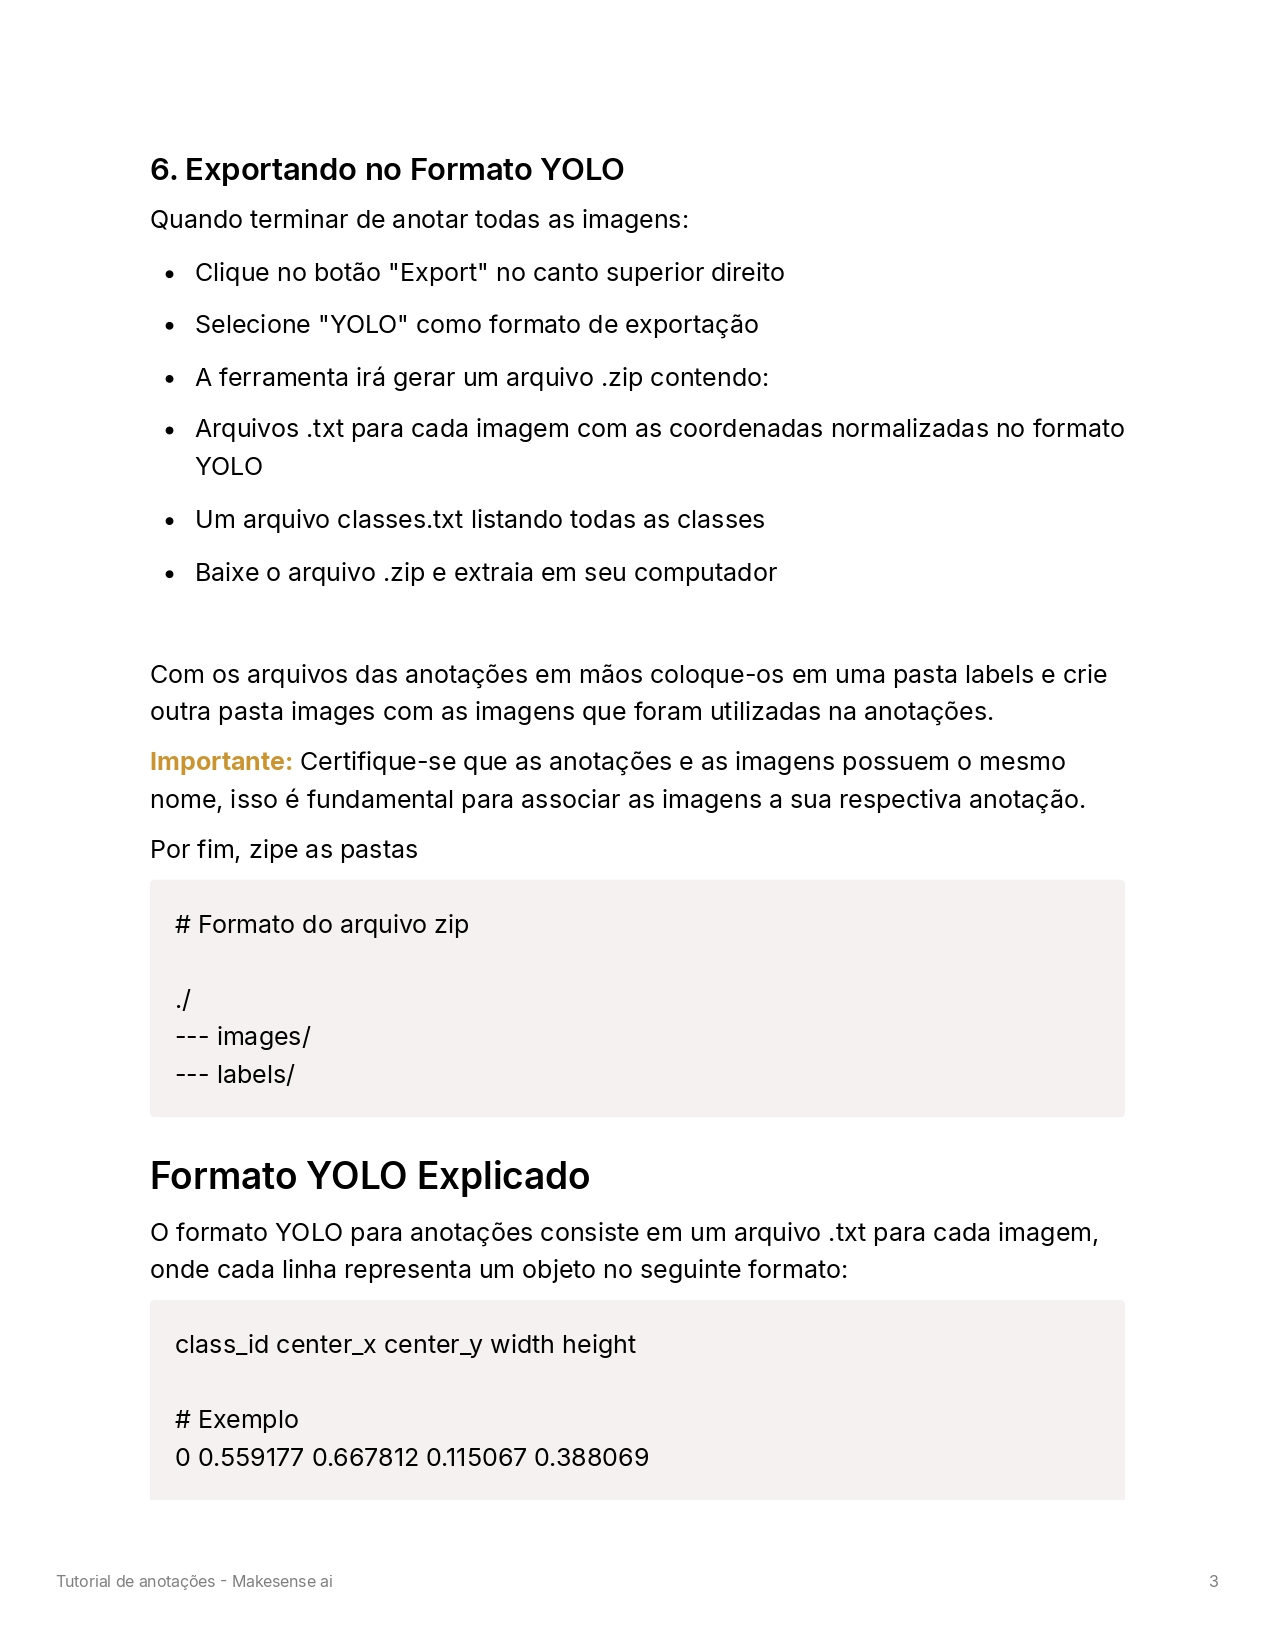
\includegraphics[width=0.8\textwidth]{./images/tutorial_p3.jpg}
    \caption{Tutorial Makesense.ai - Processo de exportação e organização de pastas.}
    \label{fig:tutorial_p3}
\end{figure}

\begin{figure}[!ht]
    \centering
    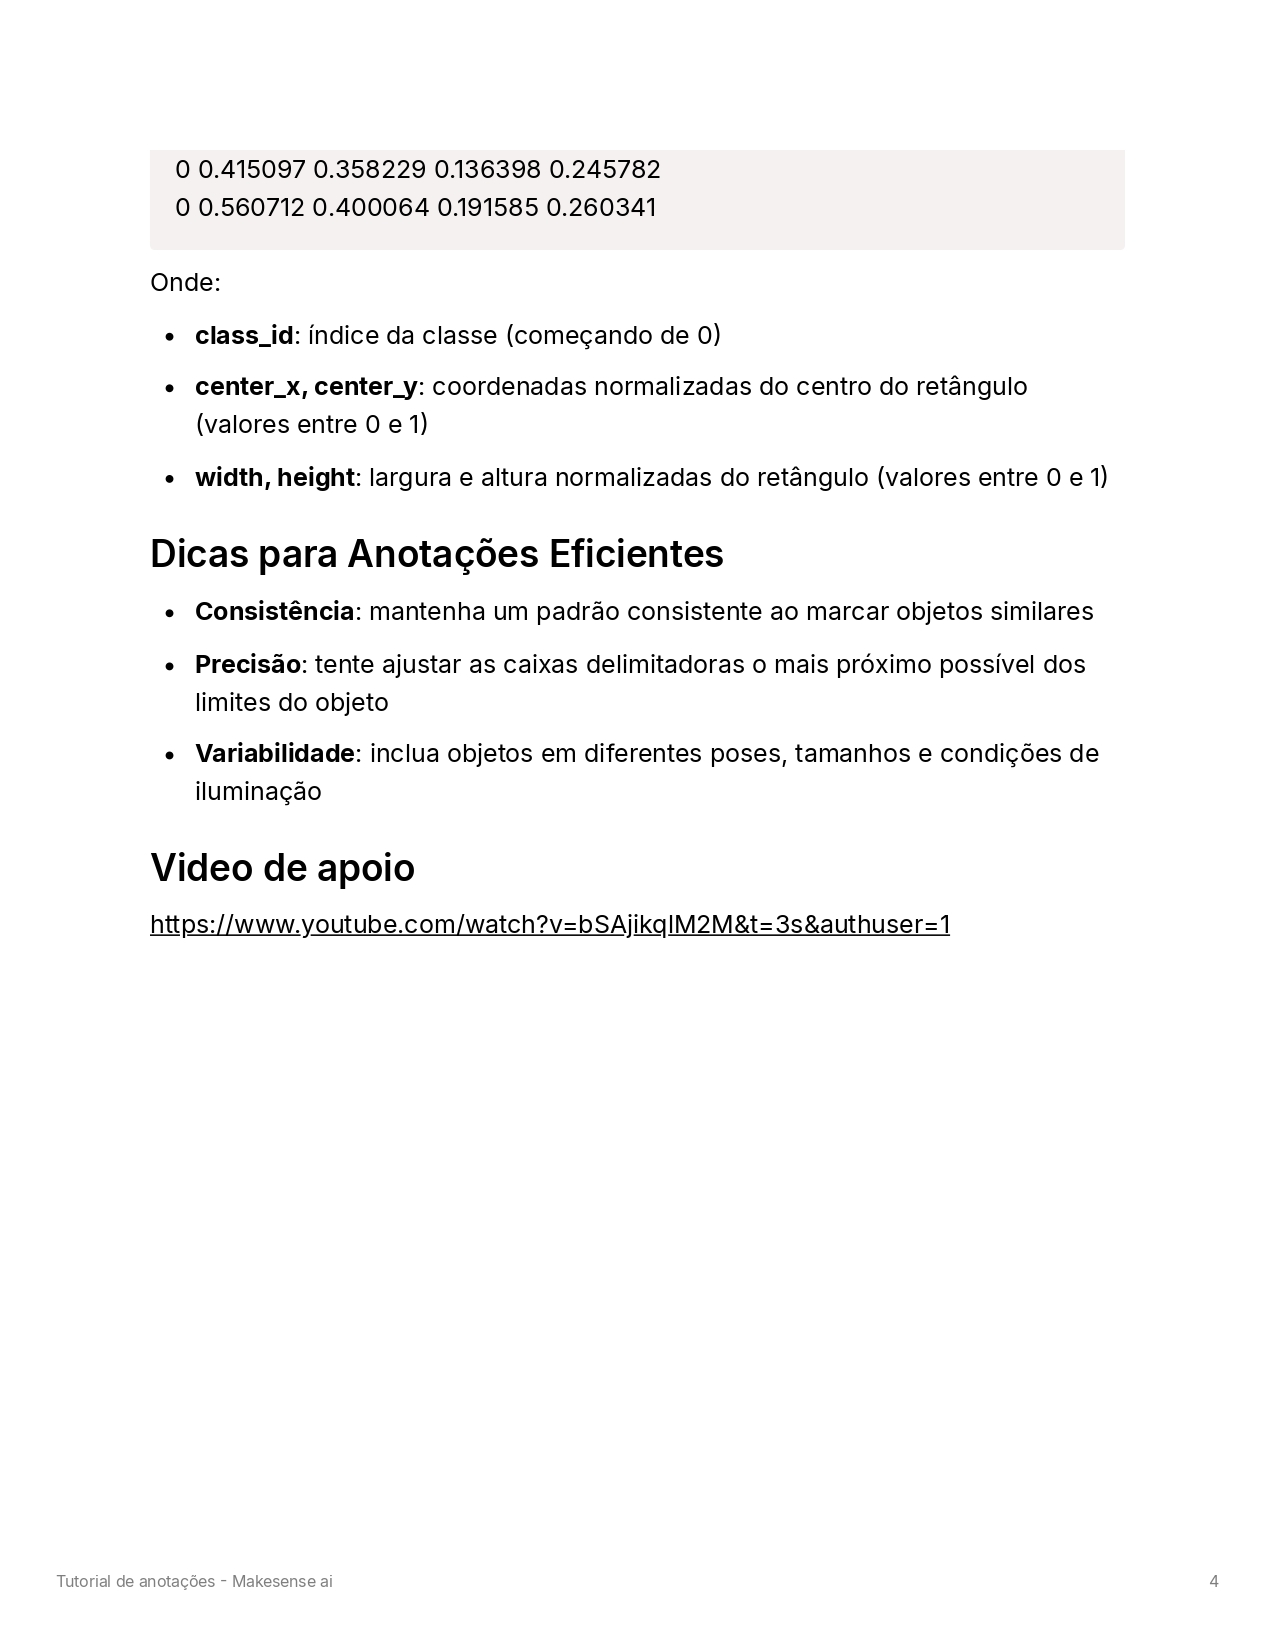
\includegraphics[width=0.8\textwidth]{./images/tutorial_p4.jpg}
    \caption{Tutorial Makesense.ai - Detalhamento técnico do formato de anotação YOLO.}
    \label{fig:tutorial_p4}
\end{figure}

\subsection{Primeiro treinamento com Dataset customizado - estudo de caso 1}
A partir do \textit{dataset} customizado, realizou-se o treinamento utilizando a versão YOLOv8, adotando uma divisão de 80\% para treino e 20\% para validação. Foram ajustados hiperparâmetros como o \textit{batch size} para -1 (otimização automática), o limite de confiança para 0,8 e o parâmetro de \textit{patience} para 30.

O processo de treinamento estendeu-se por 114 épocas, onde observou-se uma convergência estável das funções de perda (\textit{loss}). A evolução das perdas de caixa (\textit{box loss}), classificação (\textit{cls loss}) e objetividade (\textit{dfl loss}) indicou um aprendizado robusto sem sinais significativos de \textit{overfitting}, conforme ilustrado na Figura \ref{fig:grafico_losses}.

\begin{figure}[!ht]
    \centering
    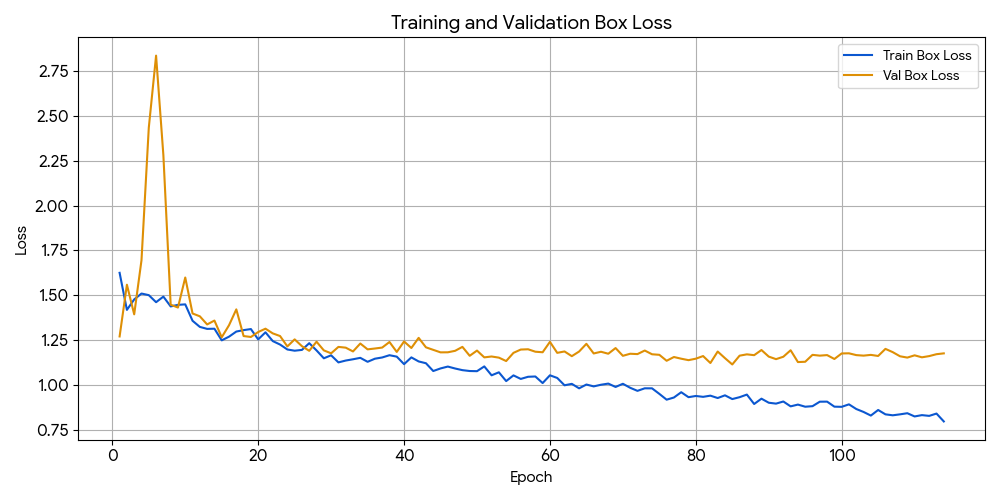
\includegraphics[width=0.8\textwidth]{./images/loss-200.png}
    \caption{Evolução das funções de perda durante as 114 épocas de treinamento.}
    \label{fig:grafico_losses}
\end{figure}

\todo{As figuras são rápidas para refazer? Se sim, aumentar a fonte dos textos dos eixos, título e legenda.} R: Preciso verificar pois tirei diretamente do PDF, posso tentar converter para doc e ajustar isso

Os resultados obtidos após o refinamento do modelo demonstraram uma alta capacidade de detecção e classificação dos caprinos. Ao final das 114 épocas, o modelo alcançou uma precisão (\textit{Precision}) de 0,9836 e uma revocação (\textit{Recall}) de 0,9812, conforme apresentado na Figura \ref{fig:grafico_pr}.

A métrica mAP50 (\textit{mean Average Precision} no limiar de 0,5) atingiu 0,9888, evidenciando a precisão do modelo na localização correta dos animais. O mAP50-95, que avalia a precisão em diferentes níveis de interseção (\textit{IoU}), consolidou-se em 0,7047. O desempenho dessas métricas ao longo do treinamento pode ser visualizado na Figura \ref{fig:grafico_map}.


\begin{figure}[!ht]
    \centering
    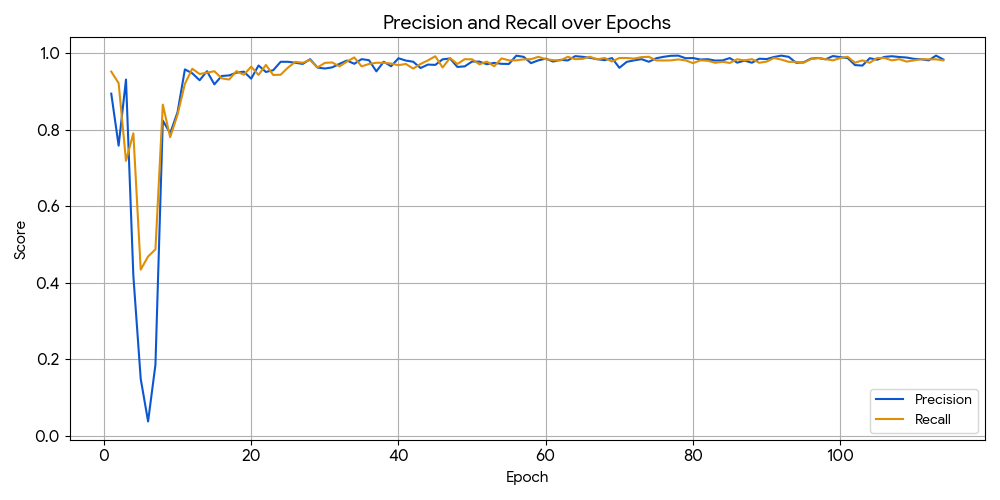
\includegraphics[width=0.8\textwidth]{./images/precision-200.png}
    \caption{Desempenho das métricas \textit{Precision} e \textit{Recall} durante o treinamento.}
    \label{fig:grafico_pr}
\end{figure}

\begin{figure}[!ht]
    \centering
    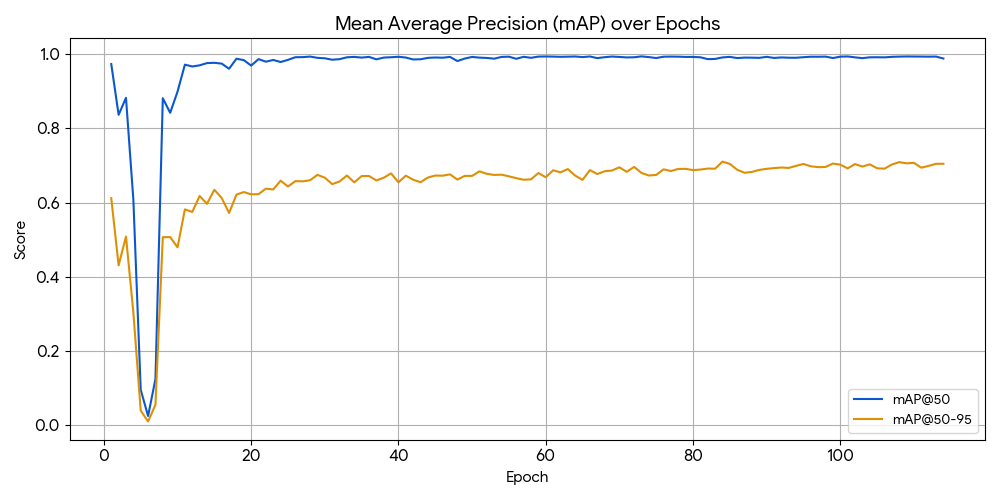
\includegraphics[width=0.8\textwidth]{./images/map-200.png}
    \caption{Evolução das métricas mAP50 e mAP50-95.}
    \label{fig:grafico_map}
\end{figure}

Estes resultados confirmam que a estratégia de especialização dos dados e o ajuste fino dos hiperparâmetros foram eficazes para superar as limitações observadas na prova de conceito e no modelo pré-treinado COCO.

Subsequentemente, realizaram-se novos experimentos com o \textit{dataset} inicial, adotando a proporção de 80/20 (treino/validação). Foram ajustados hiperparâmetros como o \textit{batch size} para -1 (otimização automática conforme a memória disponível), o limite de confiança (\textit{confidence threshold}) para 0,8 e o parâmetro de \textit{patience} para 30 (\textit{early-stopping}). Tais ajustes promoveram um refinamento significativo na classificação, em que a utilização do \textit{batch size} automático otimizou o uso da memória de vídeo, permitindo gradientes mais estáveis, enquanto o parâmetro de \textit{patience} em 30 épocas evitou o \textit{overfitting}, interrompendo o processo no ponto ideal de generalização. Como resultado, observou-se uma redução nas oscilações das funções de perda, consolidando métricas de precisão superiores a 98\%.

\subsection{Validação Cruzada e Especialização de Dados}
Como estratégia adicional para mitigar vieses decorrentes das variações de perspectiva (frontal e vertical) e iluminação (dia e noite), implementou-se a técnica de \textit{K-Fold Cross-Validation} com 5 partições (\textit{folds}). A validação cruzada (\textit{Cross-Validation}) é uma técnica estatística utilizada para avaliar a capacidade de generalização de um modelo, dividindo os dados em múltiplos subconjuntos para que cada parte seja utilizada tanto para treino quanto para teste. No caso específico do K-Fold, o conjunto de dados é particionado em k grupos (folds) de tamanhos iguais, onde o modelo é treinado k vezes, utilizando um grupo diferente como base de teste a cada iteração para garantir que todos os dados sejam validados. \todo{Explicar em 1 ou 2 frases o que é a validação cruzada.} O \textit{dataset} total foi dividido em cinco subconjuntos mutuamente exclusivos. Em cada iteração, quatro subconjuntos foram utilizados para treino e um para validação, garantindo que todos os dados fossem testados pelo menos uma vez como conjunto de validação.

Paralelamente, um segundo \textit{dataset} foi estruturado por alunos da UFSJ, que atuam como parceiros da pesquisa, segmentando as imagens por tipo (fixando perspectiva e iluminação). Os treinamentos realizados com este dado específico demonstraram que a especialização do conjunto de dados por contexto ambiental melhorou consideravelmente a precisão na detecção e classificação dos caprinos em comparação ao uso de um \textit{dataset} generalista.

\todo{Como eu comprovo essa afirmação (resultados?)}


\subsubsection{Desempenho Geral e Estabilidade}

A Tabela \ref{tab:resultados_kfold} apresenta os resultads do modelo que atingiu uma média de \textbf{99,48\%} no mAP50 e \textbf{93,15\%} no mAP50-95. O desvio padrão reduzido ($\sigma < 0,01$) entre as dobras confirma a estabilidade do treino.

\begin{table}[!ht]
\centering
\caption{Resultados detalhados da validação cruzada 5-fold.}
\label{tab:resultados_kfold}
\begin{tabular}{lcccc}
\hline
\textbf{Fold} & \textbf{mAP50} & \textbf{mAP50-95} & \textbf{\textit{Precision}} & \textbf{\textit{Recall}} \\ \hline
Fold 1 & \textbf{0,9950} & \textbf{0,9353} & 0,9976 & 0,9973 \\
Fold 2 & 0,9948 & 0,9187 & 0,9966 & 0,9986 \\
Fold 3 & 0,9947 & 0,9349 & 0,9988 & 0,9966 \\
Fold 4 & 0,9949 & 0,9339 & 0,9969 & 0,9963 \\
Fold 5 & 0,9948 & 0,9352 & 0,9997 & 0,9979 \\ \hline
\textbf{Média ($\mu$)} & \textbf{0,9948} & \textbf{0,9316} & \textbf{0,9979} & \textbf{0,9973} \\
\textbf{Desvio Padrão ($\sigma$)} & 0,0001 & 0,0072 & 0,0013 & 0,0009 \\ \hline
\end{tabular}
\end{table}

A Figura \ref{fig:map_curves-50} e \ref{fig:map_curves-50-95} ilustram a evolução das métricas de precisão média (mAP) ao longo das épocas. É possível observar uma convergência rápida e uniforme em todos os folds, além da sua estabilidade ao decorrer das épocas.

\todo{As figuras são rápidas para refazer? Se sim, aumentar a fonte dos textos dos eixos, título e legenda.}

\begin{figure}[h!]
    \centering
    \includegraphics[width=0.8\textwidth]{Template_SBC/template-latex/images/map50_k-fold.png}
    \caption{Evolução do mAP50 ao longo das épocas de treino.}
    \label{fig:map_curves-50}
\end{figure}

\begin{figure}[h!]
    \centering
    \includegraphics[width=0.8\textwidth]{Template_SBC/template-latex/images/map50-95_k-fold.png}
    \caption{Evolução do mAP50-95 ao longo das épocas de treino.}
    \label{fig:map_curves-50-95}
\end{figure}

\subsection{Análise das Curvas de Perda e Convergência}

A análise das funções de perda, apresentada na Figura \ref{fig:loss_curves}, é fundamental para verificar o desempenho \todo{Saúde? Usar uma palavra mais adequada.} do treino. Nota-se que as curvas de perda de caixa (\textit{box loss}) e classificação (\textit{cls loss}) decrescem de forma estável. A proximidade entre as curvas de treino e validação é um indicador direto da ausência de \textit{overfitting}.

\begin{figure}[h!]
    \centering
    \includegraphics[width=0.8\textwidth]{Template_SBC/template-latex/images/loss_k-fold.png}
    \caption{Curvas de perda (Loss) de treino e validação para as cinco dobras.}
    \label{fig:loss_curves}
\end{figure}

\begin{figure}[h!]
    \centering
    \includegraphics[width=0.8\textwidth]{Template_SBC/template-latex/images/box-loss-k-fold.png}
    \caption{Box Loss de treino e validação para as cinco dobras.}
    \label{fig:loss_curves}
\end{figure}

\begin{figure}[h!]
    \centering
    \includegraphics[width=0.7\textwidth]{Template_SBC/template-latex/images/fold_comparison.png}
    \caption{Comparativo de desempenho mAP50-95 por fold, evidenciando o Fold 1.}
    \label{fig:fold_comp}
\end{figure}

A interrupção antecipada (\textit{early stopping}) no Fold 1 ocorreu na época 246, garantindo que o modelo retivesse os pesos com a melhor capacidade de generalização antes de qualquer degradação por memorização do conjunto de treino.

Dentre as iterações, o \textbf{Fold 1 destacou-se como a melhor configuração}, apresentando o maior mAP50-95, 0,9353. Esta métrica é importante pois exige uma maior precisão na sobreposição das caixas delimitadoras (IoU). A Figura \ref{fig:fold_comp} compara visualmente o desempenho final entre as dobras, evidenciando o desempenho do Fold 1.

\subsection{Treinamento com dataset feito por API}

Com base nos resultados apresentados anteriormente, o uso do \textit{k-fold} juntamente com o treinamento de um modelo especializado em um tipo de imagem, apresentou bom resultado. Com isso, em parceria com os estudantes da UFSJ, foi realizado um treinamento com um \textit{dataset} gerado de forma automatizada por uma API. O objetivo desse teste foi validar se essa base de dados traria bons resultados utilizando o mesmo \textit{dataset}, pois dessa forma, pode-se garantir maior consistência entre as marcações bem como uma padronização dos dados que serão treinados.

A avaliação do desempenho do modelo ao longo dos cinco folds gerados se mostrou estável na convergência dos pesos. A métrica \textit{mean Average Precision} com limiar de interseção sobre união (\textit{Intersection over Union} - IoU) de 0,5 (mAP50) foi utilizada como o principal critério de seleção do modelo definitivo. A Tabela~\ref{tab:resultados_folds} sumariza o desempenho máximo alcançado em cada uma das rodadas.

\begin{table}[htbp]
\centering
\caption{Resultados da validação cruzada ($k$-fold) para a métrica mAP50.}
\label{tab:resultados_folds}
\begin{tabular}{cc}
\hline
\textbf{Partição (Fold)} & \textbf{mAP50 Alcançado} \\ \hline
Fold 1                   & 0,9950                   \\
Fold 2                   & 0,9950                   \\
Fold 3                   & 0,9949                   \\
Fold 4 (\textbf{Vencedor}) & \textbf{0,9950}          \\
Fold 5                   & 0,9949                   \\ \hline
\end{tabular}
\end{table}

A variação entre o menor valor registrado (0,9949) e o maior valor (0,9950) foi de apenas $0,0001$. Essa dispersão extremamente baixa evidencia que o modelo possui alta capacidade de generalização e não apresenta dependência severa da distribuição amostral de uma partição específica. 
O \textbf{Fold 4} foi determinado como o modelo vencedor por apresentar o valor teto de mAP50 igual a 0,9950.

O processo de otimização foi executado ao longo de 211 épocas. A Figura~\ref{fig:resultados_treinamento_api} ilustra o comportamento das funções de perda (\textit{loss}) e a evolução das métricas de validação ao longo do tempo.

\begin{figure}[htbp]
    \centering
    \includegraphics[width=0.9\linewidth]{Template_SBC/template-latex/images/results-api.png} 
    \caption{Curvas de perda (treinamento e validação) e evolução das métricas de desempenho ao longo das épocas.}
    \label{fig:resultados_treinamento_api}
\end{figure}

Observa-se um decréscimo acentuado e convergente nas curvas de perda de caixa (\textit{box\_loss}), perda de classe (\textit{cls\_loss}) e perda de foco de distribuição (\textit{dfl\_loss}) tanto para os dados de treinamento quanto para os de validação. Ademais, observa-se um comportamento descendente síncrono entre as perdas de treino e validação, sendo um bom indicaivo que não esta havendo \textit{overfitting} (sobreajuste), demonstrando que o processo de aprendizado está sendo efetivo.

Nas últimas épocas do treinamento, o modelo estabilizou-se com seguintes índices de desempenho:
\begin{itemize}
    \item \textbf{Precisão (Precision):} Alcançou a marca de $99,90\%$, o que reflete uma taxa quase nula de falsos positivos.
    \item \textbf{Revocação (Recall):} Estabeleceu-se em $99,69\%$, demonstrando a robustez do detector em não omitir objetos presentes na cena (falsos negativos).
    \item \textbf{mAP50-95:} Atingiu o índice de $0,9063$. Por avaliar o desempenho sob múltiplos limiares mais rigorosos de IoU (de 0,5 a 0,95), este valor superior a 90\% atesta a elevada precisão na regressão das caixas delimitadoras (\textit{bounding boxes}).
\end{itemize}


\section{Arquitetura Baseada em Mistura de Especialistas (MoE)}
\label{sec:moe_arquitetura}

A partir da validação de um modelo especializado em um tipo de imagem,foi implementada uma abordagem baseada em Mistura de Especialistas (\textit{Mixture of Experts} - MoE). Essa arquitetura fundamenta-se no princípio de ``dividir para conquistar'', onde uma rede global gerencia múltiplos submodelos especializados, direcionando cada entrada para o especialista com maior competência técnica para processá-la.

\subsection{Fundamentação Teórica e Componentes}

A arquitetura MoE proposta é composta essencialmente por dois elementos principais:

\begin{enumerate}
    \item \textbf{Rede de Roteamento (\textit{Gating Network}):} Atua como o mecanismo de decisão central do sistema. Ao receber uma imagem de entrada, a rede de roteamento calcula coeficientes de probabilidade (pesos) que determinam qual ou quais especialistas são os mais adequados para a tarefa.
    \item \textbf{Modelos Especialistas (\textit{Expert Networks}):} Conjunto de redes neurais profundas independentes, em que cada uma foi previamente submetida a um treinamento especializado em um subconjunto específico do domínio de dados (como o modelo otimizado e validado na Seção anterior).
    
\end{enumerate}

Matematicamente, para uma dada imagem de entrada $x$, a saída final do sistema $y$ é obtida pela soma ponderada das saídas de cada especialista $E_i(x)$, multiplicada pelo peso atribuído pela rede de roteamento $G(x)_i$:

\begin{equation}
y = \sum_{i=1}^{N} G(x)_i E_i(x)
\end{equation}

Onde $N$ representa o número total de especialistas disponíveis no ecossistema e $\sum G(x)_i = 1$. Para otimizar o custo computacional em tempo de execução (\textit{inference time}), o roteador foi configurado sob a estratégia \textit{Top-1 Routing}, ativando estritamente o especialista de maior afinidade e mantendo os demais em estado de inatividade (\textit{sparsity}).

\subsection{Mecanismo de Direcionamento de Imagens}

O fluxo operacional do MoE desenvolvido (Figura \ref{fig:moe_arc}) para este trabalho segue o pipeline estruturado desde a captura do dado até a inferência final:

\begin{figure}[htbp]
    \centering
    \includegraphics[width=0.9\linewidth]{Template_SBC/template-latex/images/MoE.jpeg} 
    \caption{Arquitetura proposta baseada no modelo MoE}
    \label{fig:moe_arc}
\end{figure}

\begin{enumerate}
    \item \textbf{Ingestão e Pré-processamento:} A imagem é capturada e redimensionada para os padrões exigidos pelas redes convolucionais ou transformadores visuais integrados.
    \item \textbf{Inferência do Roteador:} A \textit{Gating Network} extrai \textit{embeddings} globais da imagem para identificar seu contexto, aplicando uma função \textit{Softmax} para gerar uma distribuição de probabilidade sobre os especialistas.
    \item \textbf{Ativação Esparsa e Chaveamento:} O sistema chaveia o fluxo de dados exclusivamente para o especialista vencedor. Isso evita que todos os parâmetros de todos os modelos sejam carregados simultaneamente na memória de processamento gráfico (GPU), reduzindo a latência.
    \item \textbf{Predição Especializada:} O especialista selecionado (por exemplo, o modelo otimizado do \textit{Fold 4}) executa a detecção de objetos de alta precisão com os pesos previamente consolidados.
\end{enumerate}

Esta modularidade confere ao sistema alta escalabilidade. Caso novos cenários de detecção ou novas classes sejam adicionados futuramente ao escopo do projeto, basta treinar um novo especialista isolado e atualizar os parâmetros da rede de roteamento, dispensando a necessidade de reprocessar e retreinar todo o pipeline do zero.

\bibliographystyle{sbc}
\bibliography{sbc-template}


\end{document}
